\documentclass[notheorems]{beamer}
\usepackage{SlideStyle}
\usepackage{mathtools}
\usepackage{graphicx}
\newcommand{\Binom}{\operatorname{Binom}}
\renewcommand{\d}{\operatorname{d}}

\titlegraphic{\vspace*{-7cm}
    \parbox[c]{3cm}{
\includegraphics[height=.7cm]{bsulogo}}
    \hspace*{1cm}%
    \parbox[c]{2cm}{
\includegraphics[height=0.6cm]{FPMIlogo_new}}
    \hspace*{1cm}%
    \vspace*{3cm}
}

\title[Модели распространения заболеваний]{Дипломная работа \\ \Large CТАТИСТИЧЕСКИЙ АНАЛИЗ МОДЕЛЕЙ РАСПРОСТРАНЕНИЯ ЗАБОЛЕВАНИЙ}


\author[В. А. Гут]{Гут Валерия Александровна}

\institute[]{Научный руководитель: С.В. Лобач}


\date[]{}%{\scriptsize \structure{2017-2018}}


\begin{document}

\begin{frame}[plain]
  \titlepage
\end{frame}


%--------------------------------------------------------------------------------------
\begin{frame}{Цели и задачи работы}
	
\textbf{Объект исследования} -- распространение гриппа в Беларуси.

\textbf{Цели исследования}:

1) подготовка обзора по дифференциальным моделям распространения заболеваний;

2) подготовка обзора вероятностных, пространственных и мультиагентных популяционных моделей распространения заболеваний;

3) компьютерная реализация численных алгоритмов; сравнительный анализ построенных алгоритмов;

4) построение математических моделей распространения заболеваний с целью последующего применения этих моделей на данных Беларуси.

\textbf{Методы исследования} -- дифференциальные модели, вероятностные и пространственные методы, численные методы.
	


\end{frame}

\begin{frame}
	{Базовая модель SIR}
	В задачах моделирования процессов распространения заболеваний классической моделью является \textbf{<<Susceptible-Infected-Recovered>> (SIR)}. Эта модель формулируется в виде системы обыкновенных дифференциальных уравнений, и она отражает количество восприимчивых к заболеванию $S(t)$, инфицированных $I(t)$ и переболевших $R(t)$ людей в момент времени $t$ с учетом того, что общая популяция остается постоянной
	\begin{equation}
		S+I+R = N = \operatorname{const}.
	\end{equation} 
	
\end{frame}

\begin{frame}
	{Задача Коши для модели SIR}
		Формально, математическая модель процесса распространения заболеваний записывается в виде задачи Коши
	\begin{equation}
		\label{sir}
		\begin{dcases}
			\dfrac {\d S(t)}{\d t} = - \beta \cdot I(t)\cdot S(t),\\
			\dfrac{\d I(t)}{\d t} =\beta \cdot S(t)\cdot I(t) - \gamma\cdot I(t),\\
			\dfrac{\d R(t)}{\d t} = \gamma\cdot I(t),\\
			S(0) = S_0,\ I(0) = I_0,\ R(0) = 0.
		\end{dcases}
	\end{equation}
	Эта задача Коши описывает, как количество людей в каждой группе изменяется с течением времени. 
	
	Данная задача Коши является корректно поставленной, а ее решение предпочтительнее строить с помощью численных методов, поскольку аналитическое решение для нее записать достаточно проблематично.
	
	Путем добавления новых переменных или новых слагаемых в систему \eqref{sir} можно строить модификации для базовой модели SIR, которые расширяют возможности этой модели.
\end{frame}

\begin{frame}
	{Модификации модели SIR}
	 Например:
	\begin{itemize}
		\item если после выздоровления человек не получил иммунитет к заболеванию, то этот процесс описывает модель 
		\begin{figure}
			\centering
			
\includegraphics[scale=0.15]{images/img02}
			\caption{Модель Susceptible-Infected-Susceptible}
			\label{fig:img02}
		\end{figure}
		
		\item если человек в процессе инфицирования может умереть, то этот процесс описывает модель 
		\begin{figure}
			\centering
			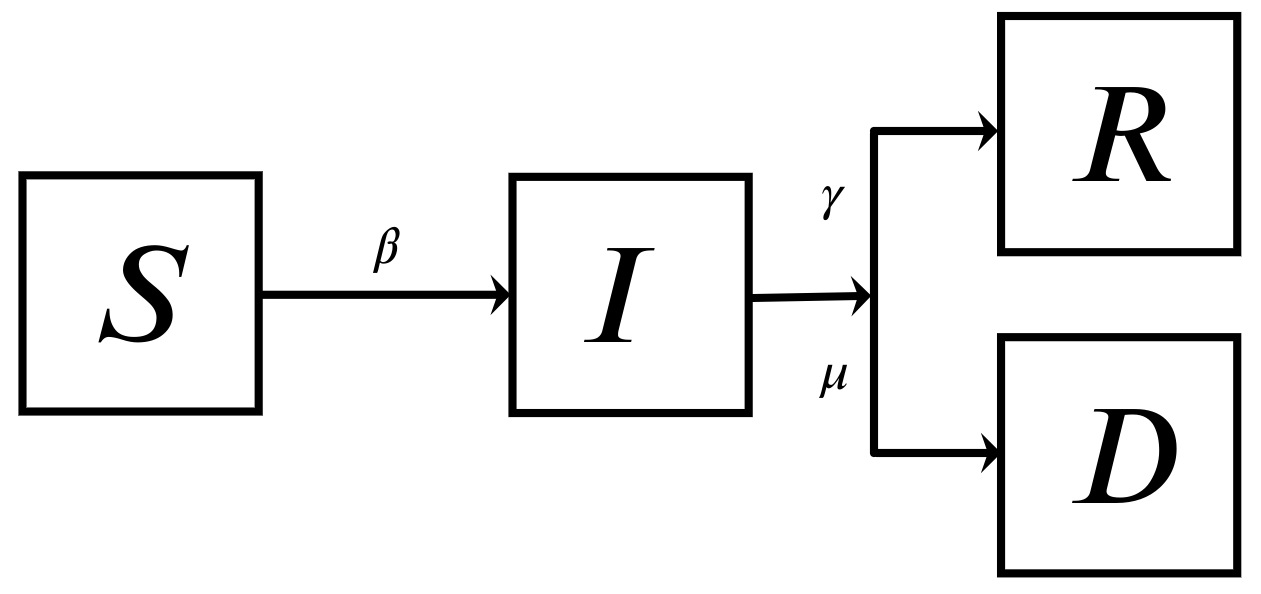
\includegraphics[scale=0.15]{images/img03}
			\caption{Susceptible-Infected-Recovered-Dead}
			\label{fig:img03}
		\end{figure}
		
	\end{itemize}
\end{frame}

\begin{frame}
	{Модификации модели SIR}
	\begin{itemize}
		\item если после выздоровления человек может потерять иммунитет к заболеванию, то этот процесс описывает модель
		\begin{figure}
			\centering
			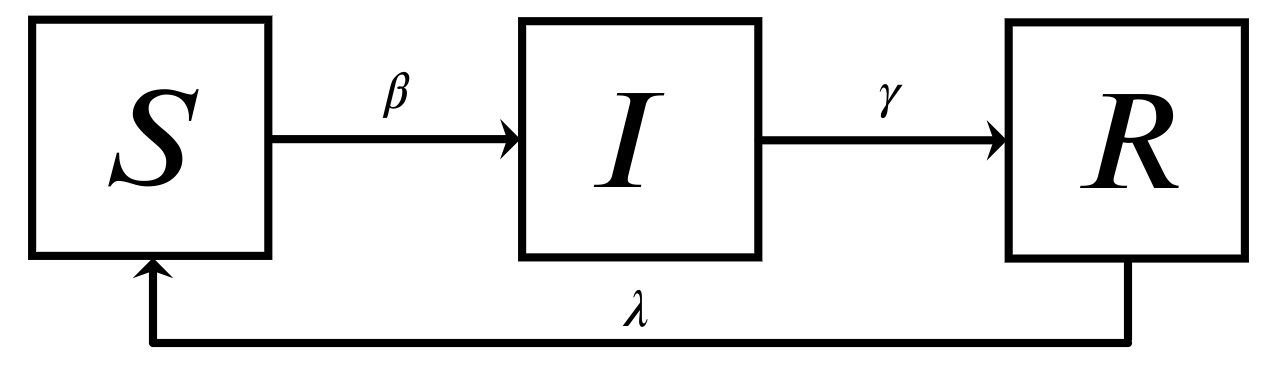
\includegraphics[scale=0.15]{images/img07}
			\caption{Модель Susceptible-Infected-Recovered-Susceptible}
			\label{fig:img07}
		\end{figure}
		
		\item инфекция имеет инкубационный период, в течение которого люди инфицированы, но не заразны, то этот процесс описывает модель 
		\begin{figure}
			\centering
			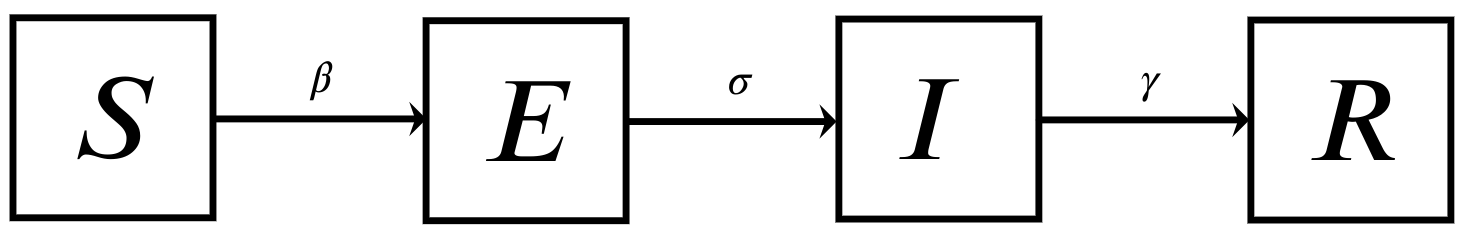
\includegraphics[scale=0.15]{images/img08}
			\caption{Модель Susceptible-Exposed-Infected-Recovered}
			\label{fig:img08}
		\end{figure}
		
	\end{itemize}
\end{frame}

%--------------------------------------------------------------------------


\begin{frame}
	{SEIR-модель}
	\small{В SEIR модели предполагается, что инфекция имеет инкубационный период, в течение которого люди инфицированы, но
	еще не заразны. Эта группа людей обозначается через $E$ (exposed). С учетом нового класса получаем следующую структуру
	популяции:
	$$S + E + I + R = N,$$ где
	\begin{itemize}
		\item $S(t)$ -- это количество не инфицированных людей, $\beta$ -- это скорость передачи заболевания;
		\item $E(t)$ -- это число инфицированных, но еще не заразных людей.  Параметр $\sigma^{-1}$ представляет собой среднюю продолжительность инкубационного периода;
		\item $I(t)$ -- это количество инфицированных людей. Параметр $\gamma$ -- это скорость восстановления;
		\item $R(t)$ -- это группа выздоровевших лиц, а именно людей, которые восстановились.
	\end{itemize}
}
\end{frame}




%--------------------------------------------------------------------------

\begin{frame}
	{SEIR-модель}
	Классическая SEIR-модель описывается задачей Коши
	Модель SEIR описывается задачей Коши
	\begin{equation*}
		\begin{dcases}
			\dfrac {\d S(t)}{\d t} = - \beta \cdot I(t)\cdot S(t),\\
			\dfrac {\d E(t)}{\d t} = \beta \cdot S(t)\cdot I(t) - \sigma\cdot E(t),\\
			\dfrac{\d I(t)}{\d t} =\sigma \cdot E(t) - \gamma\cdot I(t),\\
			\dfrac{\d R(t)}{\d t} = \gamma\cdot I(t),\\
			S(0) = S_0,\ I(0) = I_0,\ E(0) = 0,\ R(0) = 0.
		\end{dcases}
	\end{equation*}
	Эту SEIR-модель мы будем называть \textit{детерминированной} и на ее основе будет производиться решение прикладной задачи.
	
\end{frame}


\begin{frame}
	{Вероятностные популяционные модели}
	Существует другой класс расширений базовых моделей, который также увеличивает моделируемые возможности:
	\begin{itemize}
		\item замена постоянных переходов $\beta, \gamma, \sigma$ на переходы с некоторым вероятностями образует класс \textbf{вероятностных моделей}; в зависимости от распределения вероятностные модели могут быть как \textbf{дискретными}, так и \textbf{непрерывными};
	\end{itemize}
\end{frame}

\begin{frame}
	{Вероятностные популяционные модели}
			\begin{table}[h]
		\renewcommand{\arraystretch}{1}
		\caption{Сравнение дискретной и непрерывной SEIR-моделей}
		\begin{tabular}{|p{3cm}|p{3cm}|p{3cm}|}
			\hline
			\textbf{Характеристика} & \textbf{Дискретное время} & \textbf{Непрерывное время} \\ \hline
			Обновление состояния & Состояние обновляется на каждом шаге \( t \) & Состояние меняется как процесс Пуассона \\ \hline
			Применение & Удобна для численного моделирования & Более точна для моделирования реального времени \\ \hline
			Интенсивности переходов & Вероятности событий за шаг времени & Скорости событий (интенсивности) \\ \hline
		\end{tabular}
	\end{table}
\end{frame}


%--------------------------------------------------------------------------


\begin{frame}
	{Моделирование процесса распространения гриппа. Постановка задачи
	}
	\textbf{Сформулирована задача моделирования процесса распространения гриппа в Беларуси.}
	Симптомы гриппа появляются на \textbf{1—4-й день} после заражения и включают в себя лихорадку, кашель, головную боль, боль в мышцах и суставах, слабость, боль в горле и насморк. При этом кашель может длиться две и более недели. Наиболее заразен больной на \textbf{3—4-й день} с момента появления симптомов. Реконвалесцентный период составляет \textbf{7—15 дней}. После выздоровления формируется иммунитет к конкретному штамму вируса, но он не защищает от других штаммов. Иммунитет носит временный характер (обычно до \textbf{1-2 лет}).
\end{frame}

\begin{frame}
	{Входные данные}
\small {На основе приведенной информации о распространении можем сформулировать математическую модель следующим образом. Так как симптомы появляются через 1-4 дня, то возьмем средний инкубационный период для модели $T_\text{инкубац} = 2$ дня. Тогда коэффициент перехода из $E$ в $I$ равна
$$\sigma = \dfrac{1}{T_\text{инкубац}} = \dfrac 1 2 = 0.5.$$
Средний инфекционный период выберем $T_\text{инфекц}=5$ дней.
Тогда коэффициент выздоровления равен
$$\gamma = \dfrac{1}{T_\text{инфекц}} = \dfrac 1 5 = 0.2.$$
Коэффициент передачи инфекции $\beta$ мы можем получить из  базового репродуктивного числа через следующее соотношение
$$\beta = R_0\cdot \gamma = 1.5\cdot 0.2 = 0.3.$$

В качестве числа населения возьмем $N=1000$, а число инфицированных зададим равное $I_0 = 20$. Отсюда $S_0 = N - I_0 = 980$. Данный процесс будем рассматривать в течение $T=100$ дней.}
\end{frame}

%--------------------------------------------------------------------------

\begin{frame}
	{Применение детерминированной SEIR модели для моделирования}
	Ввиду входных условий, получаем систему дифференциальных уравнений модели SEIR
	\begin{equation*}
		\begin{dcases}
			\dfrac {\d S(t)}{\d t} = - 0.3 \cdot I(t)\cdot S(t),\\
			\dfrac {\d E(t)}{\d t} = 0.3 \cdot S(t)\cdot I(t) - 0.5\cdot E(t),\\
			\dfrac{\d I(t)}{\d t} =0.5 \cdot E(t) - 0.2\cdot I(t),\\
			\dfrac{\d R(t)}{\d t} = 0.2\cdot I(t),\\
			S(0) = 980,\ I(0) = 20,\ E(0) = 0,\ R(0) = 0.
		\end{dcases}
	\end{equation*} 
	
	Ее решение вычисляется с помощью численных методов.
\end{frame}

%--------------------------------------------------------------------------
\begin{frame}
	{Применение детерминированной SEIR модели для моделирования}
\begin{figure}
	\centering
	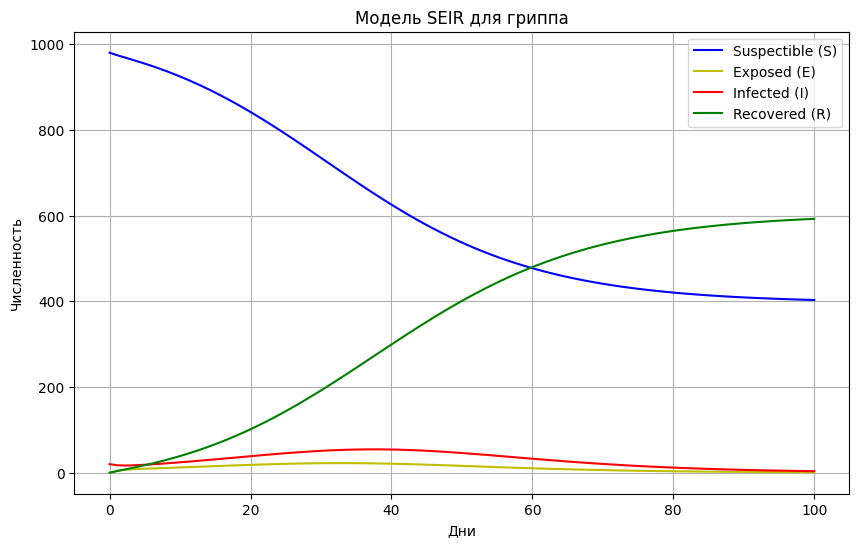
\includegraphics[scale=0.4]{images/graph01}
	\caption{График численного решения задачи Коши для детерминированной SEIR модели}
	\label{fig:graph01}
\end{figure}
\end{frame}

%--------------------------------------------------------------------------

\begin{frame}
	{Вероятностные популяционные модели}
	\small{Построим вероятностную модель с дискретным временем, поскольку для нее легко привести численную реализацию. Вероятностная SEIR-модель для гриппа имеет следующий вид
	\begin{equation}
		\begin{dcases}
			S_{t+1} = S_t - \Delta E_t,\\
			E_{t+1} = E_t +\Delta E_t - \Delta I_t,\\
			I_{t+1} = I_t + \Delta I_t - \Delta R_t,\\
			R_{t+1} = R_t + \Delta R_t,
			S_0 = 980,\ E_0 = 0,\ I_0 = 20,\ \ R_0 = 0
		\end{dcases}
		t = 0,1,2\ldots,
	\end{equation}
	при этом
	$$\Delta E_t \sim \Binom\left(S_t, 
	1 - \exp\left(-\beta\cdot  \frac{I}{N} \cdot \Delta t\right)\right),$$
	$$\Delta I_t \sim \Binom\left(E_t, 1 - \exp\left(-\sigma \cdot \Delta t\right)\right),$$
	$$\Delta R_t \sim \Binom\left(I_t, 1 - \exp\left(-\gamma \cdot \Delta t\right)\right).$$
	
	Таким образом, мы можем описать процесс распространения гриппа с помощью вероятностной SEIR модели. Приведем 100 реализаций этой модели, а в качестве результирующего графика выберем средние значения для каждой группы, а также приведем 95\%-доверительные интервалы для каждой переменной}
\end{frame}

%--------------------------------------------------------------------------

\begin{frame}
	{Вероятностные популяционные модели}
	\begin{figure}
		\centering
		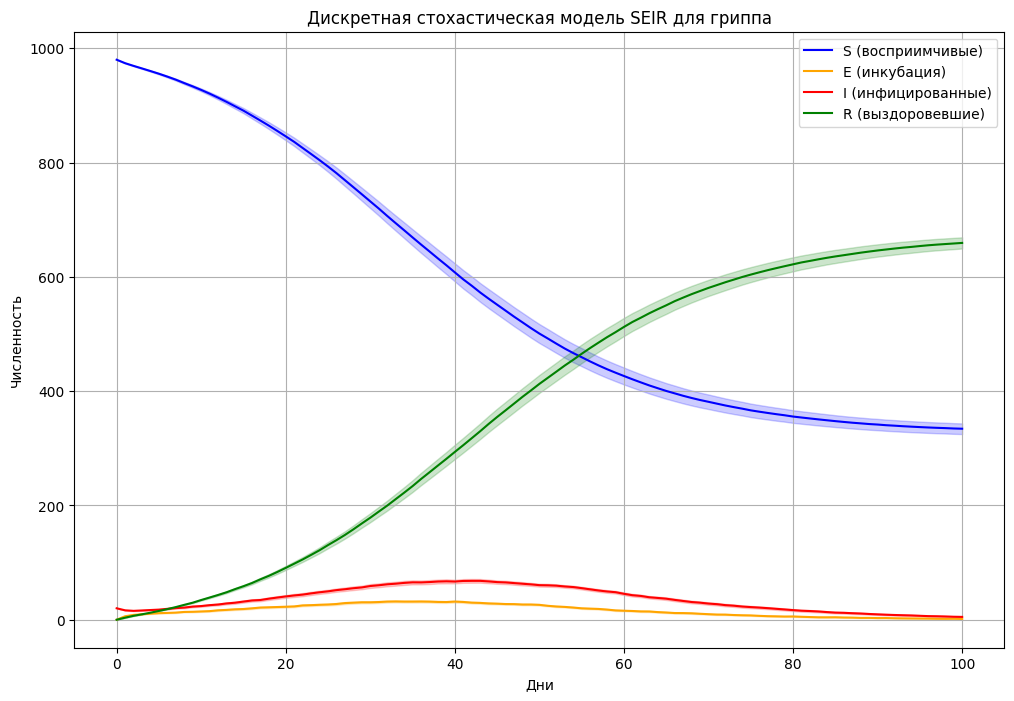
\includegraphics[scale=0.4]{images/graph02}
		\caption{График численной реализация вероятностной SEIR для гриппа с доверительными интервалами}
		\label{fig:graph02}
	\end{figure}
	
\end{frame}

%--------------------------------------------------------------------------

\begin{frame}
	{Постановка задачи для пространственной модели}
	Клеточные автоматы -- это удобный инструмент для моделирования пространственных процессов, таких как распространение инфекции. В такой модели
	
	\begin{itemize}
		\item пространство делится на дискретные ячейки (регион, квартал, город и т.д.);
		\item каждая ячейка имеет состояние (например, $S$, $E$, $I$, $R$);
		\item состояние каждой ячейки обновляется во времени в зависимости от её текущего состояния и состояния соседей.
	\end{itemize}
	
	Клеточные автоматы хорошо подходят для моделирования локальных взаимодействий и пространственного распространения инфекции.
\end{frame}
%--------------------------------------------------------------------------

\begin{frame}{Применение пространственной SEIR модели для моделирования}
	\small{Для пространственной модели построим сетку узлов $30 \times 30$ на которой зададим вероятностную SEIR-модель для дискретного времени с сохранением всех параметров из предыдущего случая. Клетки, в которых будут находиться инфицированные люди, будут выбираться случайно.}
	
	
\end{frame}

%--------------------------------------------------------------------------

\begin{frame}
	
	{Применение пространственной SEIR модели для моделирования}
	\begin{figure}
		\centering
		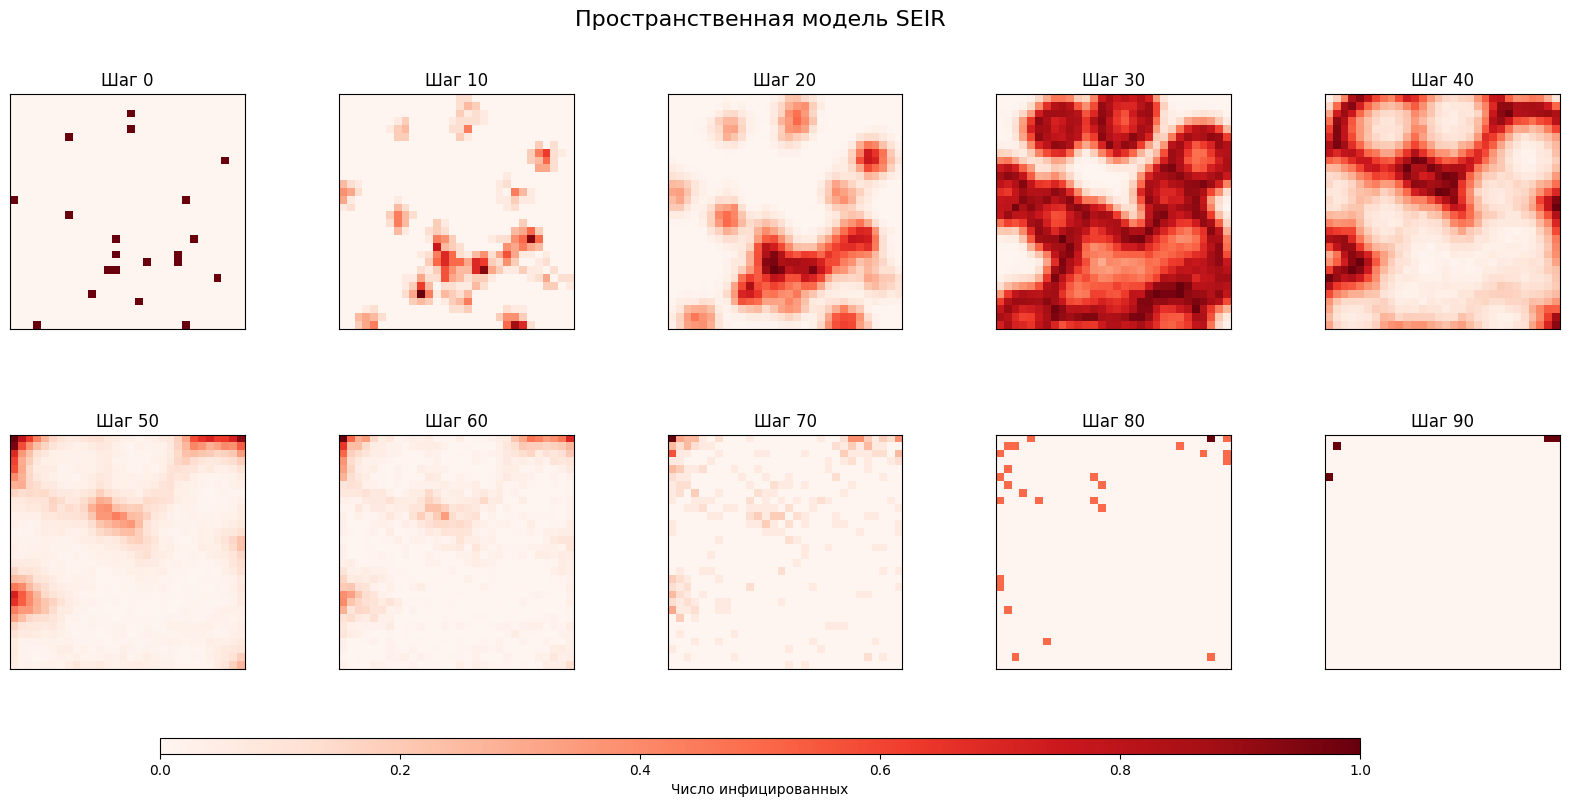
\includegraphics[scale=0.3]{images/graph03}
		\caption{Пространственные графики численной реализации вероятностной SEIR модели для гриппа}
		\label{fig:graph03}
	\end{figure}
	
\end{frame}

%--------------------------------------------------------------------------



\begin{frame}
	{Индивидуум-ориентированные и мультиагентные методы моделирования}
	\small{В модели, построенной на основе клеточных автоматов, используется решетка, где каждая ячейка представляет собой часть популяции. Однако в реальности индивиды имеют различные характеристики, например
	\begin{itemize}
		\item индивидуальная восприимчивость, то есть люди имеют разный иммунитет, что влияет на вероятность заражения;
		\item различные периоды инкубации и выздоровления, то есть у разных индивидов инкубационный и инфекционный периоды могут варьироваться;
		\item индивидуальные контакты, то есть люди взаимодействуют с разным числом других людей, что влияет на передачу болезни;
		\item мобильность, то есть люди перемещаются в пространстве (не фиксированы в одной ячейке).
	\end{itemize}
	
	Учет этих факторов может значительно повысить точность модели, так как она будет учитывать вариативность в поведении и характеристиках индивидов.}
\end{frame}

%--------------------------------------------------------------------------

\begin{frame}
	{Индивидуум-ориентированные и мультиагентные методы моделирования}
\begin{figure}
	\centering
	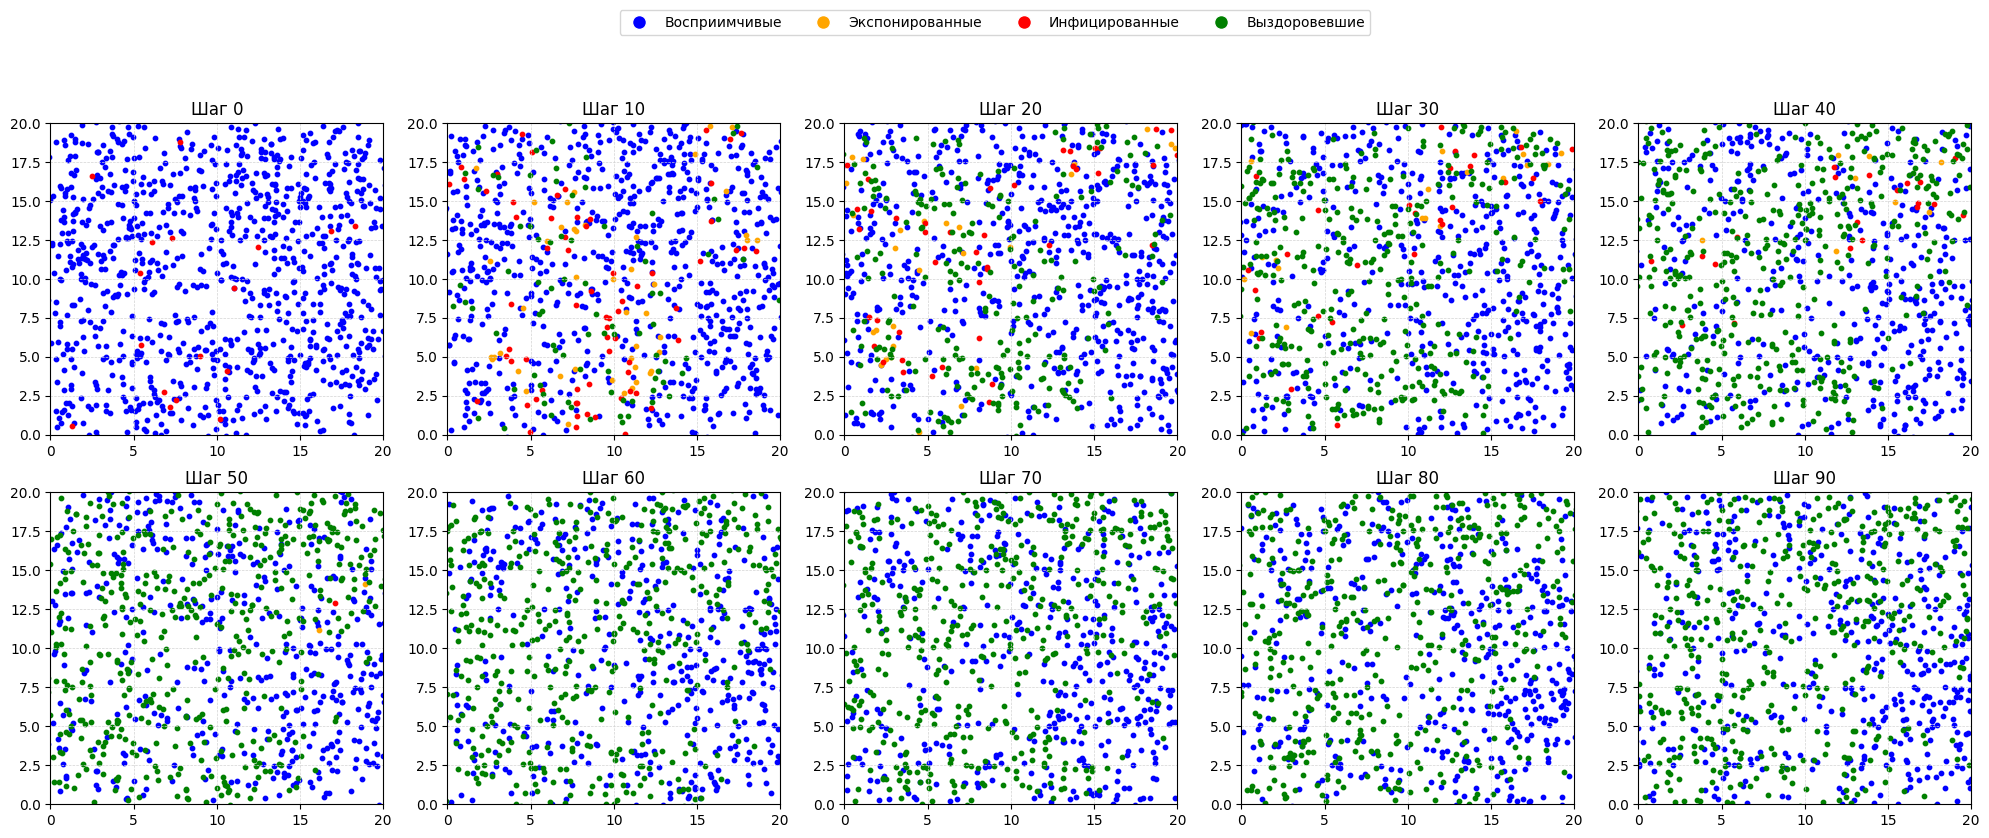
\includegraphics[scale=0.2]{images/graph04}
	\caption{Графическое представление реализации мультиагентной SEIR модели}
	\label{fig:graph04}
\end{figure}
\end{frame}

%--------------------------------------------------------------------------

\begin{frame}
	{Заключение}
	В данной работе рассмотрена SEIR-модель и ее расширения, с помощью которых был смоделирован процесс распространения заболеваний.
В ходе работы
\begin{enumerate}
	\item рассмотрена классическая SI-модель и ее аналитическое решение;
	\item рассмотрена классическая SIR-модель, вывод ее дифференциальных уравнений, исследование вопроса о корректной постановке задачи Коши, построение аналитического решения, описание методов построения приближенного решения;
	\item рассмотрены основные базовые модификации SIR-модели: SIS, SIRS, SIRD, SEIR, MSIR, MSEIR;
	\item рассмотрены расширения базовой SEIR модели: вероятностная модель, пространственная модель, мультиагентная модель;
	\item на практике были рассмотрены способы построения расширений для модели SEIR для решения задачи о моделировании распространения гриппа и приведены результаты моделирования.
\end{enumerate}
\end{frame}

%--------------------------------------------------------------------------

\begin{frame}
	{Список используемых источников}
	\begin{enumerate}
		\item Детерминированные и стохастические модели распространения инфекции и тестирование в изолированном контингенте/ Чигарев, А. В.,Журавков, М. А.,Чигарев, В. А.// Журнал Белорусского государственного университета. Математика. Информатика - 2021. - № 3. - С. 57-67
		\item Methods of intellectual data analysis in COVID-19 research / O. V. Senko, A. V. Kuznetsova, E. M. Voronin, O. A. Kravtsova, L. R. Borisova, I. L. Kirilyuk, V. G. Akimkin// Journal of the Belarusian State University. Mathematics and Informatics. – 2022. – № 1. – С. 83-96
		\item Statistical forecasting of the dynamics of epidemiological indicators for COVID-19 incidence in the Republic of Belarus / Yu. S. Kharin, V. A. Valoshka, O. V. Dernakova, V. I. Malugin, A. Yu. Kharin// Journal of the Belarusian State University. Mathematics and Informatics. - 2020. - № 3. - С. 36-50
		
		
	\end{enumerate}
\end{frame}

%--------------------------------------------------------------------------

\begin{frame}
	\begin{center}
		\huge{Спасибо за внимание!}
	\end{center}
\end{frame}

\end{document} 